\mode*		%% Reset Mode

\section{A Worked Example}

\mode<presentation>
\begin{frame}
	\frametitle{Putting it all Together}
	Let's try to recreate this diagram:

	\begin{columns}[T]
		\begin{column}{.5\textwidth}
			\centering
			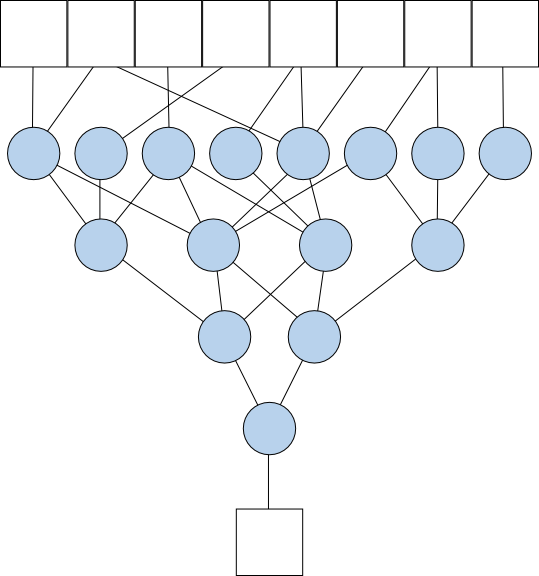
\includegraphics[width=\textwidth]{figures/specification}
		\end{column}
		\begin{column}{.5\textwidth}
			Assume structure is constant, but connections variable.

			How do we:
			\begin{itemize}
				\item \textbf{position nodes?}
				\item place edges?
			\end{itemize}
		\end{column}
	\end{columns}
\end{frame}
\mode*

We should now be able to put everything we've learnt together to develop a more complex example.
Specifically, we'll investigate how we might implement Figure \ref{figure.worked-example.specification} in Ti\emph{k}Z.
We'll assume that the underlying structure is constant, but that we would like an easy way of modifying the connections between the nodes, such that we can have many diagrams of a similar type.
Thus, the questions we need to answer are (1) how do we position the nodes? and (2) having placed the nodes, how do we place the edges such that they are easy to change?

\begin{figure}[btp]
	\centering
	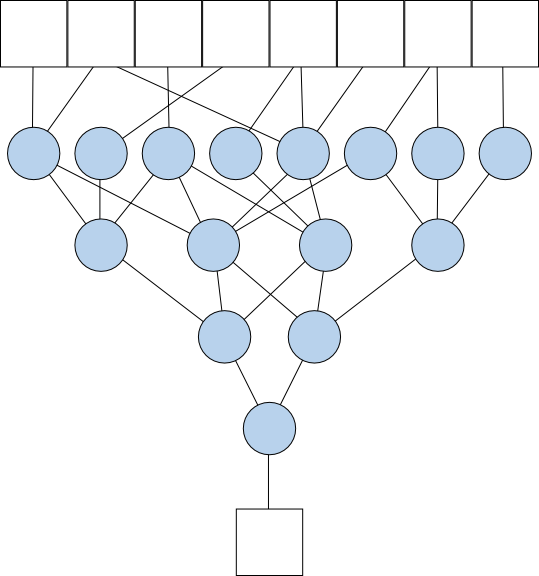
\includegraphics[width=.25\textwidth]{figures/specification}
	\caption{The figure we'd like to implement in TikZ.}
	\label{figure.worked-example.specification}
\end{figure}

As a first approximation, we may consider placing the nodes manually; though this seems unnecessarily laborious!
Listing \ref{listing.worked-example.1} illustrates how we might do this, and Figure \ref{figure.worked-example.1} shows how far I got before getting bored(!); we've also introduced the \texttt{scope} environment, this applies any options we give it to any Ti\emph{k}Z commands that fall within it.


\begin{figure}[btp]
	\centering
	\begin{subfigure}{.45\textwidth}
		\centering
		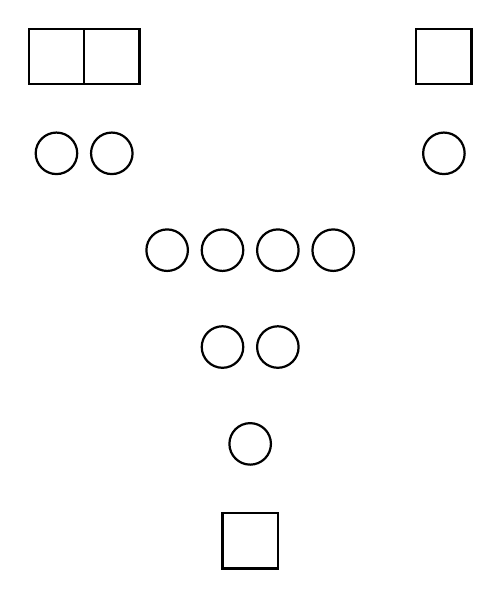
\begin{tikzpicture}

	%% The input row
	\begin{scope}[every node/.style={draw, thick, rectangle, minimum size=2em}]
		\node at ( 0em,0) (1-1) {};
		\node at ( 2em,0) (1-2) {};
		% ...
		\node at (14em,0) (1-8) {};
	\end{scope}

	%% The first row
	%% Shifted down (yshift=-...) and across (xshift=...)
	\begin{scope}[every node/.style={draw, thick, circle, minimum size=1.5em}, yshift=-3.5em]
		\node at ( 0em,0) (2-1) {};
		\node at ( 2em,0) (2-2) {};
		% ...
		\node at (14em,0) (2-8) {};
	\end{scope}

	%% The second row
	%% Shifted down (yshift=-...) and across (xshift=...)
	\begin{scope}[every node/.style={draw, thick, circle, minimum size=1.5em}, xshift=4em, yshift=-7.0em]
		\node at ( 0em,0) (3-1) {};
		\node at ( 2em,0) (3-2) {};
		\node at ( 4em,0) (3-3) {};
		\node at ( 6em,0) (3-4) {};
	\end{scope}

	%% The third row
	\begin{scope}[every node/.style={draw, thick, circle, minimum size=1.5em}, xshift=6em, yshift=-10.5em]
		\node at ( 0em,0) (4-1) {};
		\node at ( 2em,0) (4-2) {};
	\end{scope}

	%% The fourth row
	\begin{scope}[every node/.style={draw, thick, circle, minimum size=1.5em}, xshift=7em, yshift=-14.0em]
		\node at ( 0em,0) (5-1) {};
	\end{scope}

	%% The output row
	\begin{scope}[every node/.style={draw, thick, rectangle, minimum size=2em}, xshift=7em, yshift=-17.5em]
		\node at ( 0em,0) (6-1) {};
	\end{scope}

\end{tikzpicture}

		\caption{Manually placing nodes.}
		\label{figure.worked-example.1}
	\end{subfigure}
	\begin{subfigure}{.45\textwidth}
		\centering
		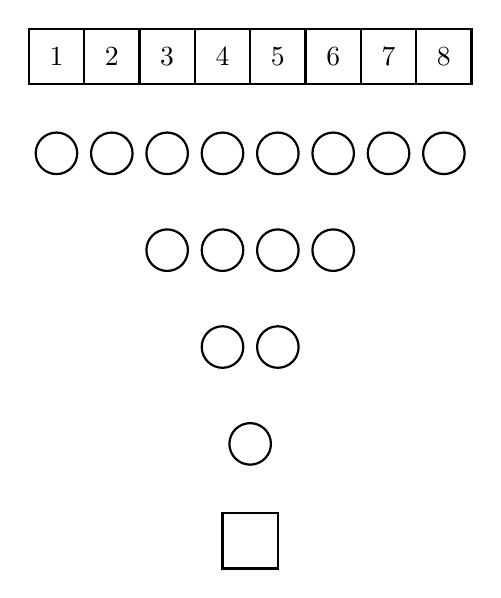
\begin{tikzpicture}

	%% The input row (index = 1)
	\begin{scope}[every node/.style={draw, thick, rectangle, minimum size=2em}]
		%% Iterate from 1-8, storing the index in \n
		\foreach \n in {1,...,8}{%
			\node at (\n*2em, 0) (1-\n) {\n};
		}
	\end{scope}

	%% Iterate through the processing rows
	%% We use a counter to track the row number
	\foreach [count=\r from 2] \m in {8, 4, 2, 1}{%
		%% Calculate the shifts using PGF math
		\pgfmathsetmacro\xShift{(8-\m)/2*2em}
		\pgfmathsetmacro\yShift{(\r-1)*-3.5em}

		\begin{scope}[every node/.style={draw, thick, circle, minimum size=1.5em}, xshift=\xShift, yshift=\yShift]
			\foreach \n in {1,...,\m}{%
				\node at (\n*2em, 0) (\r-\n) {};
			}
		\end{scope}
	}

	%% The output row
	\node at (9em,-17.5em) [draw, rectangle, thick, minimum size=2em] (6-1) {};

\end{tikzpicture}

		\caption{Using iteration to procedurally generate the nodes.}
		\label{figure.worked-example.2}
	\end{subfigure}
	\caption{Using TikZ to reproduce our target image.}
\end{figure}

\lstinputlisting[language=TeX, caption={Manual positioning of nodes.}, label={listing.worked-example.1}]{examples.article/worked-example-1.tex}

It should be obvious that there was a fair amount of unnecessary repetition when we place the nodes manually; thankfully by using PGF we can perform iteration.
The \texttt{\textbackslash foreach \textit{token} in \textit{list}\{\textit{action}\}} macro will perform \textit{action} for every item in the list.
Listing \ref{listing.worked-example.2} uses this to reduce the amount of work needed to produce the diagram, the result is shown in Figure \ref{figure.worked-example.2}.

\lstinputlisting[language=TeX, caption={Iterative positioning of nodes.}, label={listing.worked-example.2}]{examples.article/worked-example-2.tex}

This is far more concise, and would be an appropriate point to consider how to place edges.
First, however, we should note that our styles (\texttt{draw, rectangle, \ldots}) we spattered throughout our code, and it would be nice to refer to styles in terms of, say, \texttt{port} and \texttt{neuron}.
Thankfully, Ti\emph{k}Z also makes this possible!
The snippet of code shown in Listing \ref{listing.worked-example.3} creates two styles named as above, and means that we can replace lines 4 and 18 as below:\\
\texttt{\textbackslash begin\{scope\}[every node/.style=port, \ldots]}\\
\texttt{\textbackslash begin\{scope\}[every node/.style=neuron, \ldots]}

\lstinputlisting[language=TeX, caption={Creating our own styles.}, label={listing.worked-example.3}]{examples.article/worked-example-3.tex}

We should also note that we named our nodes by their row number, followed by a hyphen, followed by their number from left to right.
This will make it considerably easier to make connections between them.
Intuitively, all the code we need to link the 1st element of the 1st row with the 1st element of the 2nd row is:\\
\texttt{\textbackslash draw (1-1) to (2-1);}

Ideally, however, we would like a way of taking a list of pairs of the left-to-right number of the nodes to be connected, and then to add these arbitrary edges.
By extending the \texttt{foreach} command, this can be easily achieved.\\
\texttt{\textbackslash foreach \textbackslash x/\ldots/\textbackslash z in \{ 0/\ldots/n, \ldots \}\{\textit{actions\ldots}\}}

For example, the code in Listing \ref{listing.worked-example.4} will generate the links between the first two rows.

\lstinputlisting[language=TeX, caption={Automatically linking nodes using foreach.}, label={listing.worked-example.4}]{examples.article/worked-example-4.tex}

Even better, given a list of lists of pairs, we could generate all the links in one fell swoop; Listing \ref{listing.worked-example.5} illustrates this.

\lstinputlisting[language=TeX, caption={Automatically linking all nodes using foreach.}, label={listing.worked-example.5}]{examples.article/worked-example-5.tex}

Finally, putting all of the above together we get Listing \ref{listing.worked-example.finali}, the result of which is Figure \ref{figure.worked-example.final}.

\begin{figure}[btp]
	\begin{subfigure}{.5\textwidth}
		\centering
		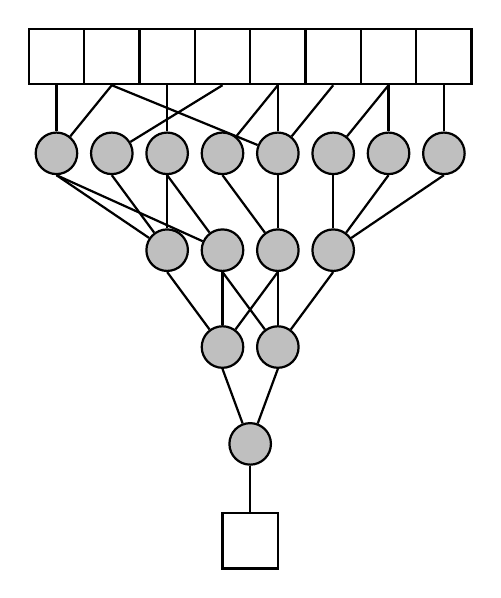
\begin{tikzpicture}[
	net node/.style = {draw, thick},
	port/.style = {net node, rectangle, minimum size=2em},
	neuron/.style = {net node, circle, minimum size=1.5em, fill=gray!50!white},
	edge/.style = {thick},
]

	%% The input row (index = 1)
	\begin{scope}
		%% Iterate from 1-8, storing the index in \n
		\foreach \n in {1,...,8}{%
			\node [port] at (\n*2em, 0) (1-\n) {};
		}
	\end{scope}

	%% Iterate through the processing rows
	%% We use a counter to track the row number
	\foreach [count=\r from 2] \m in {8, 4, 2, 1}{%
		%% Calculate the shifts using PGF math
		\pgfmathsetmacro\xShift{(8-\m)/2*2em}
		\pgfmathsetmacro\yShift{(\r-1)*-3.5em}

		\begin{scope}[xshift=\xShift, yshift=\yShift]
			\foreach \n in {1,...,\m}{%
				\node [neuron] at (\n*2em, 0) (\r-\n) {};
			}
		\end{scope}
	}

	%% The output row
	\node at (9em,-17.5em) [port] (6-1) {};

	%% Draw the connections
	%% User specified
	\foreach [count=\m] \l in {%
		{1/1, 2/1, 2/5, 3/3, 4/2, 5/4, 5/5, 6/5, 7/6, 7/7, 8/8},	% 1st to 2nd
		{1/1, 1/2, 2/1, 3/1, 3/2, 4/3, 5/3, 6/4, 7/4, 8/4},		% 2nd to 3rd
		{1/1, 2/1, 2/2, 3/1, 3/2, 4/2},					% 3rd to 4th
	}{%
		%% \m is the start row, let \n be the end row
		\pgfmathtruncatemacro\n{\m+1}	% Truncate makes an int from a float
	
		\foreach \u/\v in \l {% Here \l is one of the lists defined above
			\draw [edge] (\m-\u.south) to (\n-\v);
		}
	}

	%% Always present
	\foreach [count=\m from 4] \l in {{1/1, 2/1}, {1/1}}{%
		\pgfmathtruncatemacro\n{\m+1}	% Truncate makes an int from a float
		\foreach \u/\v in \l {% Here \l is one of the lists defined above
			\draw [edge] (\m-\u.south) to (\n-\v);
		}
	}

\end{tikzpicture}

		\caption{The final result, not quite as specified, but certainly close enough, and easily reused.}
		\label{figure.worked-example.final}
	\end{subfigure}
	\begin{subfigure}{.5\textwidth}
		\centering
		\newcommand*{\neuralnetdiagram}[1]{% A new command called \neuralnetdiagram with 1 parameter `#1'
\begin{tikzpicture}[
	net node/.style = {draw, thick},
	port/.style = {net node, rectangle, minimum size=2em},
	neuron/.style = {net node, circle, minimum size=1.5em, fill=gray!50!white},
	edge/.style = {thick},
]

	%% The input row (index = 1)
	\begin{scope}
		%% Iterate from 1-8, storing the index in \n
		\foreach \n in {1,...,8}{%
			\node [port] at (\n*2em, 0) (1-\n) {};
		}
	\end{scope}

	%% Iterate through the processing rows
	%% We use a counter to track the row number
	\foreach [count=\r from 2] \m in {8, 4, 2, 1}{%
		%% Calculate the shifts using PGF math
		\pgfmathsetmacro\xShift{(8-\m)/2*2em}
		\pgfmathsetmacro\yShift{(\r-1)*-3.5em}

		\begin{scope}[xshift=\xShift, yshift=\yShift]
			\foreach \n in {1,...,\m}{%
				\node [neuron] at (\n*2em, 0) (\r-\n) {};
			}
		\end{scope}
	}

	%% The output row
	\node at (9em,-17.5em) [port] (6-1) {};

	%% Draw the connections
	%% User specified
	\foreach [count=\m] \l in {#1}{% This uses our parameter
		%% \m is the start row, let \n be the end row
		\pgfmathtruncatemacro\n{\m+1}	% Truncate makes an int from a float
	
		\foreach \u/\v in \l {% Here \l is one of the lists defined above
			\draw [edge] (\m-\u.south) to (\n-\v);
		}
	}

	%% Always present
	\foreach [count=\m from 4] \l in {{1/1, 2/1}, {1/1}}{%
		\pgfmathtruncatemacro\n{\m+1}	% Truncate makes an int from a float
		\foreach \u/\v in \l {% Here \l is one of the lists defined above
			\draw [edge] (\m-\u.south) to (\n-\v);
		}
	}

\end{tikzpicture}
}

		\neuralnetdiagram{%
			{1/1, 1/2, 2/1, 2/3, 3/3, 3/4, 4/4, 5/5, 6/6, 8/6, 8/7, 8/8},%
			{1/1, 2/1, 3/1, 3/2, 4/2, 5/4, 6/3, 6/4, 7/3, 8/4},%
			{1/1, 2/1, 3/2, 4/2},%
		}
		\caption{The result of the macro to generate a different network connectivity.}
	\end{subfigure}
	\caption{The results of our labours.}
\end{figure}

Having mentioned reuse as desirable, a good question is, can we wrap this in a macro that accepts the list of connections as a parameter and then draws the network?
The answer, unsurprisingly, is \textit{yes}.
Listing \ref{listing.worked-example.finalii} shows how we'd modify the code to make a macro, and then we can draw the diagram with \texttt{\textbackslash neuralnetdiagram\{\textit{list}\}}.

\lstinputlisting[language=TeX, caption={The final result.}, label={listing.worked-example.finali}]{examples.article/worked-example-finali.tex}
\lstinputlisting[language=TeX, caption={The final result, modified to produce a parametrised macro.}, label={listing.worked-example.finalii}]{examples.article/worked-example-finalii.tex}

\mode<all>	%% Reset mode again
